\chapter{Thermodynamique des piles électrochimiques}\label{ch:b2:cell-thermodynamics}

Un bus à pile à hydrogène transporte un empilement de quelques centaines de cellules minces. Dans chacune,
le dihydrogène et le dioxygène de l'air se combinent en eau sans flamme, et
l'énergie en sort sous forme de courant électrique. Deux nombres gouvernent un tel empilement, et
tous deux sortent directement des tables d'\omterm{def:b2:reaction-free-energy:gibbs-energy}{enthalpies libres}~: aucune cellule ne peut donner plus de
\qty{1.23}{V}, et aucune pile à combustible, si parfaite soit-elle, ne transforme toute l'énergie de son
dihydrogène en travail électrique. Ce chapitre relie la tension d'une pile à
l'\omterm{def:b2:reaction-free-energy:gibbs-energy}{enthalpie libre} de sa réaction, établit la relation de Nernst utilisée depuis le
volume de première année, et tire d'un voltmètre et d'un thermomètre les entropies et les \omterm{def:b2:reaction-enthalpy:reaction-quantity}{enthalpies de réaction}.

\begin{recall}
Le volume de première année~: piles, demi-piles, anode et cathode, pont salin, tension
de la pile, potentiel d'électrode, potentiel standard et électrode standard à
hydrogène, relation de Nernst (admise alors), constantes d'équilibre à partir des
potentiels. \Cref{ch:b2:reaction-free-energy}~: $\Delta_r G$, $\Delta_r G^\circ$
et $\Delta_r G = \Delta_r G^\circ + RT\ln Q$~; le critère d'évolution.
\Cref{ch:b2:chemical-potential}~: les activités. Le volume scolaire~: l'électrolyse.
\end{recall}

\begin{omfigure}
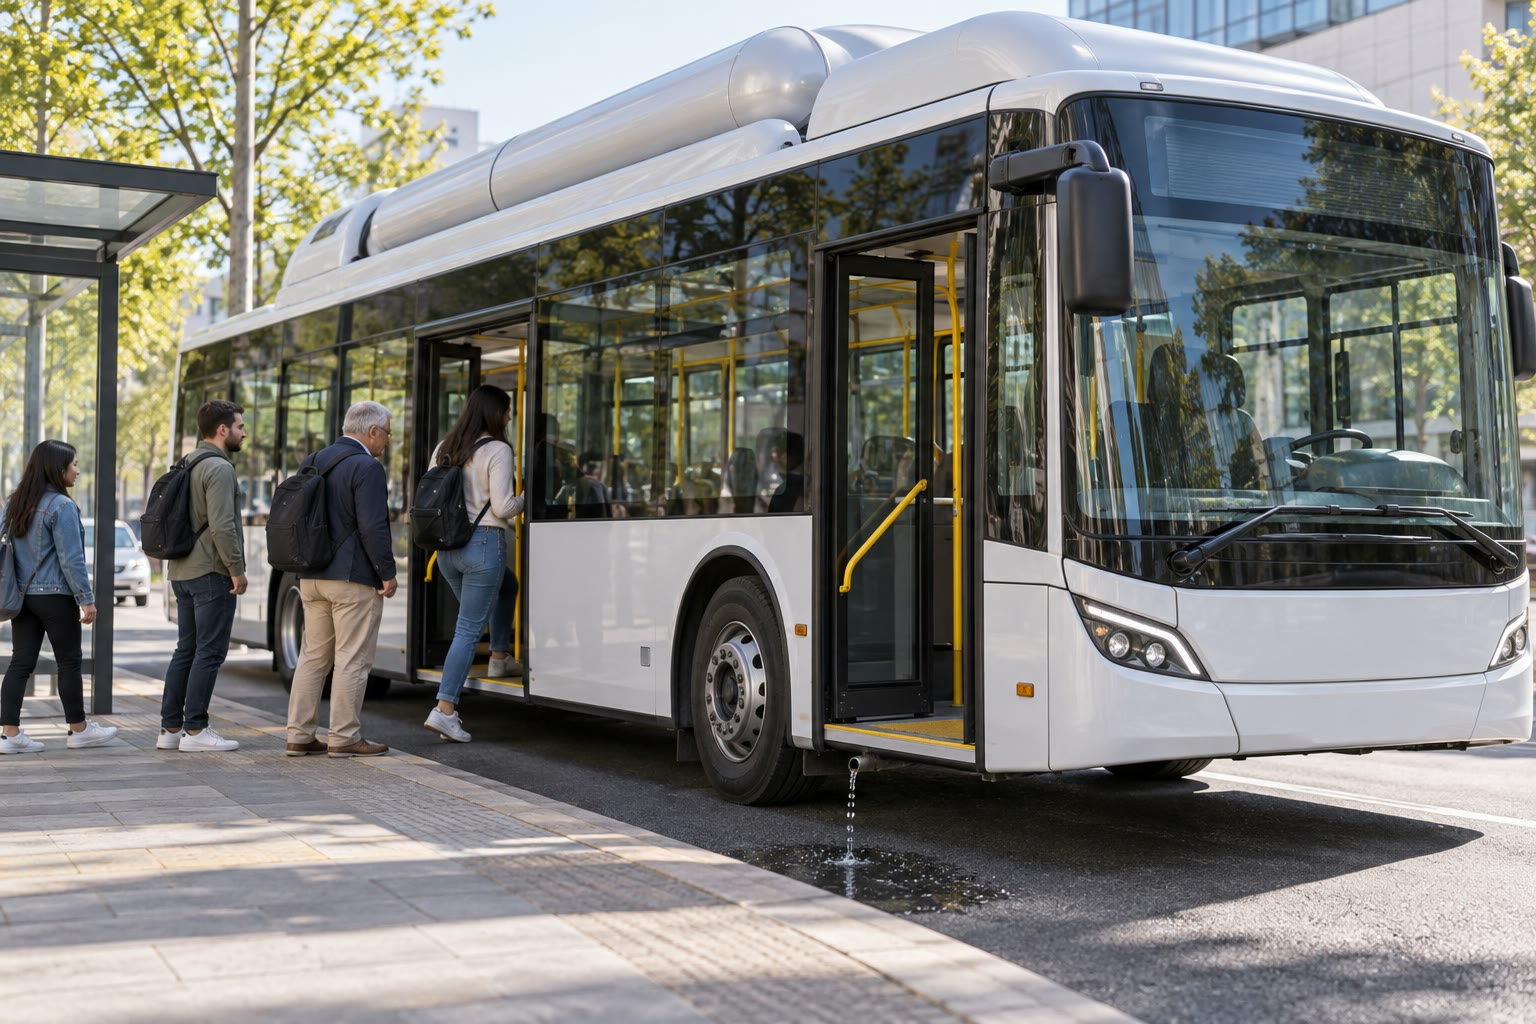
\includegraphics[width=0.62\linewidth]{images/book3/ai/b2-09-fuel-cell-bus.jpg}

{\small Un bus à pile à hydrogène à un arrêt~: les réservoirs de dihydrogène sont sous le
carénage du toit, et le seul rejet est de l'eau, qui goutte sous le bus.}
\end{omfigure}

\section{Travail électrique et constante de Faraday}

\begin{definition}[Constante de Faraday]\label{def:b2:cell-thermodynamics:faraday}
La \emph{constante de Faraday}\index{constante de Faraday} est la charge électrique
d'une mole de charges élémentaires, $F = N_A e = \qty{96485.33}{C/mol}$.
% ledger: const:F
\end{definition}

\begin{proposition}[Charge débitée]\label{prop:b2:cell-thermodynamics:charge}
Si la réaction d'une pile, écrite avec $n$ électrons échangés, avance de
$\Delta\xi$, la charge qui traverse le circuit extérieur est $Q =
nF\,\Delta\xi$.
\end{proposition}

\begin{proof}
Un avancement $\Delta\xi$ transfère $n\,\Delta\xi$ moles d'électrons de
l'anode vers la cathode par le fil, chacun de charge $e$ en valeur absolue~:
$Q = n\,\Delta\xi\,N_A e$.
\end{proof}

Lorsqu'une charge $Q$ est mise en mouvement dans un circuit par une tension $U$, le travail
reçu par le circuit est $QU$. Du point de vue de la pile, qui fournit ce travail,
le travail électrique qu'elle reçoit est $\delta W_{\text{él}} = -U\,\delta Q = -nFU\,
d\xi$.

\begin{omfigure}
\begin{tikzpicture}[font=\small, >={Stealth}]
  \draw[thick, rounded corners, fill=omDef!8] (0,0) rectangle (3.2,2.2);
  \node[align=center] at (1.6,1.1) {pile\\ (système)\\ réaction $d\xi$};
  \draw[->, thick, omThm] (3.2,1.6) -- (5.6,1.6) node[right, align=left] {$\delta W_{\text{él}}$ fourni\\ $= nFU\,d\xi$};
  \draw[->, thick, omDef] (5.6,0.6) -- (3.2,0.6) node[pos=0, right, align=left] {$\delta Q_{\text{th}}$ reçu\\ (de signe quelconque)};
  \draw[<->, thick] (1.6,2.2) -- (1.6,3.0) node[above] {milieu extérieur à $T$, $p$};
\end{tikzpicture}

{\small Une pile vue comme un système thermodynamique à température et pression constantes~:
elle échange de la chaleur avec le milieu extérieur et fournit un travail électrique par
le circuit extérieur. Avec la convention de signe du premier principe (travail et chaleur
reçus comptés positivement), $\delta W_{\text{él}} = -nFU\,d\xi$.}
\end{omfigure}

\section{L'enthalpie libre d'une réaction de pile}

\begin{theorem}[Travail électrique et enthalpie libre]\label{thm:b2:cell-thermodynamics:delta-g-nfe}
Une pile fonctionnant à $T$ et $p$ constantes fournit un travail électrique au plus
égal à la diminution de son \omterm{def:b2:reaction-free-energy:gibbs-energy}{enthalpie libre}~: pour un avancement $d\xi$,
$nFU\,d\xi \leq -\Delta_r G\,d\xi$. Lorsqu'elle fonctionne de façon réversible (courant
infinitésimal), l'égalité est vérifiée, et la tension de la pile est la
force électromotrice
\[
  \Delta_r G = -nFE .
\]
\end{theorem}

\begin{proof}
Premier principe à pression constante, le travail des forces de pression étant mis à part~:
$dH = \delta Q + \delta W_{\text{él}}$. Second principe~: $dS \geq \delta Q/T$. À
$T$ et $p$ constantes, $dG = dH - T\,dS \leq \delta W_{\text{él}} = -nFU\,d\xi$.
Avec $dG = \Delta_r G\,d\xi$, $\Delta_r G\,d\xi \leq -nFU\,d\xi$, c'est-à-dire
$nFU\,d\xi \leq -\Delta_r G\,d\xi$. Pour une transformation réversible, l'inégalité
du second principe devient une égalité, et la tension alors mesurée, à courant
nul, est $E$~: $\Delta_r G = -nFE$.
\end{proof}

Une pile ne peut donc fonctionner dans le sens direct ($d\xi > 0$, en fournissant du travail) que si $\Delta_r G <
0$, c'est-à-dire $E > 0$, les pôles étant choisis de sorte que la réaction écrite se déroule
de l'anode vers la cathode. Une pile réelle, traversée par un courant, fournit
moins de travail que $-\Delta_r G$~: la différence est dissipée en chaleur dans sa
résistance et à ses électrodes (\cref{ch:b2:current-potential-curves}).

\begin{example}[La pile Daniell]\label{ex:b2:cell-thermodynamics:daniell}
Pour \ce{Zn + Cu^2+ -> Zn^2+ + Cu}, $\Delta_r G^\circ = \Delta_f G^\circ(\ce{Zn^2+}) -
\Delta_f G^\circ(\ce{Cu^2+}) = -147.06 - 65.49 = \qty{-212.55}{kJ/mol}$, et $n = 2$~:
$E^\circ = 212\,550/(2 \times 96\,485) = \qty{1.10}{V}$, la tension mesurée sur une
pile Daniell dans les conditions standard.
% ledger: dfg:Zn2+_ao, dfg:Cu2+_ao, const:F, emf:Daniell
\end{example}

\section{La relation de Nernst et les potentiels standard}

Le volume de première année avait admis la relation de Nernst~; elle découle maintenant de
$\Delta_r G = \Delta_r G^\circ + RT\ln Q$.

\begin{theorem}[La relation de Nernst, démontrée]\label{thm:b2:cell-thermodynamics:nernst-derived}
Pour une demi-équation $\alpha\,\mathrm{Ox} + n\,\mathrm e^- \rightleftharpoons
\beta\,\mathrm{Red}$, le potentiel de l'électrode à la température $T$ vaut
\[
  E = E^\circ + \frac{RT}{nF}\ln\frac{a_{\mathrm{Ox}}^{\alpha}}{a_{\mathrm{Red}}^{\beta}} ,
\]
où les activités comprennent celles de toutes les autres espèces de la
demi-équation (\ce{H+}, l'eau exceptée), affectées de leurs puissances stœchiométriques.
\end{theorem}

\begin{proof}
Le potentiel d'une électrode est la tension de la pile formée de l'électrode standard à
hydrogène (anode) et de cette électrode (cathode). Sa réaction est
\[
  \alpha\,\mathrm{Ox} + \tfrac n2\,\ce{H2} \longrightarrow \beta\,\mathrm{Red} + n\,\ce{H+} ,
\]
dont le quotient de réaction, avec $a_{\ce{H+}} = 1$ et $p_{\ce{H2}} = p^\circ$ à
l'électrode standard à hydrogène, se réduit à $a_{\mathrm{Red}}^\beta/
a_{\mathrm{Ox}}^\alpha$. D'après le \cref{thm:b2:cell-thermodynamics:delta-g-nfe},
$E = -\Delta_r G/(nF) = -\Delta_r G^\circ/(nF) - (RT/nF)\ln Q$~; avec $E^\circ =
-\Delta_r G^\circ/(nF)$, c'est la formule. À \qty{298.15}{K}, $RT\ln 10/F =
\qty{0.0592}{V}$.
\end{proof}

\begin{proposition}[Potentiels standard et enthalpies libres]\label{prop:b2:cell-thermodynamics:standard-potential}
Avec les conventions $\Delta_f G^\circ(\ce{H+}, \text{aq}) = 0$ et
$\Delta_f G^\circ(\ce{H2}, \text{g}) = 0$, le potentiel standard d'un couple est
$E^\circ = -\Delta_r G^\circ/(nF)$, où $\Delta_r G^\circ$ est l'\omterm{def:b2:reaction-free-energy:gibbs-energy}{enthalpie libre}
standard de la demi-équation écrite dans le sens de la réduction, les électrons étant comptés
avec une \omterm{def:b2:reaction-free-energy:gibbs-energy}{enthalpie libre} nulle.
\end{proposition}

\begin{proof}
Dans la réaction contre l'électrode à hydrogène, $\tfrac n2\,\ce{H2}$ et
$n\,\ce{H+}$ n'apportent rien à $\Delta_r G^\circ$ avec ces conventions~: l'\omterm{def:b2:reaction-free-energy:gibbs-energy}{enthalpie
libre} standard de la réaction de pile est celle de la seule demi-équation.
\end{proof}

\begin{method}[Un potentiel standard à partir des tables]\label{met:b2:cell-thermodynamics:e-from-gibbs}
\begin{enumerate}
  \item Écrire la demi-équation dans le sens de la réduction, équilibrée avec \ce{H+} et
        \ce{H2O}, avec $n$ électrons.
  \item Calculer $\Delta_r G^\circ = \sum\nu_i\Delta_f G^\circ_i$ (produits
        comptés positivement), avec zéro pour les éléments, \ce{H+} et les électrons.
  \item $E^\circ = -\Delta_r G^\circ/(nF)$, en volts avec $\Delta_r G^\circ$ en
        joules par mole.
\end{enumerate}
\end{method}

\begin{example}[L'électrode au chlorure d'argent]\label{ex:b2:cell-thermodynamics:agcl}
\ce{AgCl(s) + e- -> Ag(s) + Cl^-}~: $\Delta_r G^\circ = -131.228 - (-109.789) =
\qty{-21.439}{kJ/mol}$, $E^\circ = 21\,439/96\,485 = \qty{0.222}{V}$. Son potentiel
ne dépend que de l'activité des ions chlorure~: dans une solution saturée de chlorure de
potassium, c'est une électrode de référence stable.
% ledger: dfg:Cl-_ao, dfg:AgCl_cr
\end{example}

\begin{proposition}[Combiner des potentiels]\label{prop:b2:cell-thermodynamics:combining}
Si une demi-équation (3), à $n_3$ électrons, est la somme des demi-équations (1)
et (2), à $n_1$ et $n_2$ électrons, alors
\[
  n_3E_3^\circ = n_1E_1^\circ + n_2E_2^\circ ;
\]
les potentiels eux-mêmes ne s'additionnent pas.
\end{proposition}

\begin{proof}
Les \omterm{def:b2:reaction-free-energy:gibbs-energy}{enthalpies libres} standard s'additionnent, $\Delta_r G_3^\circ = \Delta_r G_1^\circ + \Delta_r
G_2^\circ$, et les nombres d'électrons aussi, $n_3 = n_1 + n_2$. Il reste à diviser chaque $\Delta_r
G^\circ$ par $-F$.
\end{proof}

\begin{example}[Le fer à ses deux nombres d'oxydation]\label{ex:b2:cell-thermodynamics:iron}
\ce{Fe^3+ + e- -> Fe^2+} a pour $E^\circ = (-78.90 + 4.7)/(-96.485) = \qty{0.77}{V}$
et \ce{Fe^2+ + 2e- -> Fe} a pour $E^\circ = -78.90/(2 \times 96.485) =
\qty{-0.41}{V}$. D'où, pour \ce{Fe^3+ + 3e- -> Fe}~: $E^\circ = (0.77 - 0.82)/3 =
\qty{-0.02}{V}$, et non la somme des deux.
% ledger: dfg:Fe2+_ao, dfg:Fe3+_ao
\end{example}

\section{Température, entropie et rendement d'une pile à combustible}

\begin{definition}[Coefficient de température]\label{def:b2:cell-thermodynamics:temperature-coefficient}
Le \emph{coefficient de température}\index{coefficient de temperature@coefficient de température} d'une pile est
la dérivée $(\partial E/\partial T)_p$ de sa force électromotrice par
rapport à la température.
\end{definition}

\begin{proposition}[Entropie et enthalpie à partir des données de la pile]\label{prop:b2:cell-thermodynamics:entropy}
Pour la réaction de pile standard,
\[
  \Delta_r S^\circ = nF\,\frac{dE^\circ}{dT}, \qquad
  \Delta_r H^\circ = -nF\Big(E^\circ - T\frac{dE^\circ}{dT}\Big),
\]
et une pile fonctionnant de façon réversible à la température $T$ reçoit du
milieu extérieur la chaleur $T\Delta_r S$ par mole de réaction.
\end{proposition}

\begin{proof}
$\Delta_r S^\circ = -d\Delta_r G^\circ/dT$ (d'après $dG = -S\,dT + V\,dp$, dérivée
par rapport à $\xi$) $= nF\,dE^\circ/dT$~; puis $\Delta_r H^\circ = \Delta_r G^\circ
+ T\Delta_r S^\circ$. Pour la transformation réversible, $\delta Q = T\,dS = T\Delta_r S\,
d\xi$.
\end{proof}

\begin{method}[Des données de la pile à la thermodynamique de la réaction]\label{met:b2:cell-thermodynamics:cell-data}
\begin{enumerate}
  \item Mesurer $E$ à plusieurs températures~; la pente est $dE/dT$.
  \item $\Delta_r G = -nFE$, $\Delta_r S = nF\,dE/dT$, $\Delta_r H = \Delta_r G +
        T\Delta_r S$.
  \item Chaleur échangée par mole lorsque la pile fonctionne de façon réversible~: $T\Delta_r S$~;
        lorsqu'elle débite un courant sous une tension $U < E$, la chaleur libérée vaut
        $-\Delta_r H - nFU$ par mole.
\end{enumerate}
\end{method}

Pour la pile dihydrogène--dioxygène produisant de l'eau liquide, les valeurs clés du CODATA
donnent $\Delta_r H^\circ = \qty{-285.83}{kJ/mol}$ et
\[
  \Delta_r S^\circ = 69.95 - 130.68 - \tfrac12 \times 205.15 = \qty{-163.3}{J/(K.mol)} ,
\]
donc $\Delta_r G^\circ = \qty{-237.14}{kJ/mol}$ et $E^\circ = \qty{1.229}{V}$~; le
\omterm{def:b2:cell-thermodynamics:temperature-coefficient}{coefficient de température} vaut $\Delta_r S^\circ/(2F) = \qty{-0.85}{mV/K}$. Une pile à hydrogène donne une tension
plus faible à chaud qu'à froid.
% ledger: dfh:H2O-l, s0:H2O_l, s0:H2_g, s0:O2_g, janafG:H2O_l.298

\begin{omfigure}
\begin{tikzpicture}
\begin{axis}[width=0.48\linewidth, height=5.4cm, xmin=280, xmax=1020,
  ymin=0.95, ymax=1.26, axis x line=bottom, axis y line=left,
  xlabel={$T$ (K)}, ylabel={$E^\circ$ (V)}, tick label style={font=\small},
  label style={font=\small}, title={\small tension standard}]
\addplot[omDef, thick, mark=*, mark size=1.2pt] table[x=T, y=E] {figdata/out/bachelor-2-cell-thermodynamics-a-liquid.dat};
\addplot[omThm, thick, mark=*, mark size=1.2pt] table[x=T, y=E] {figdata/out/bachelor-2-cell-thermodynamics-a-gas.dat};
\node[font=\scriptsize, omDef, anchor=north east] at (axis cs:480,1.05) {eau liquide};
\node[font=\scriptsize, omThm, anchor=south west] at (axis cs:560,1.12) {vapeur d'eau};
\end{axis}
\end{tikzpicture}\hfill
\begin{tikzpicture}
\begin{axis}[width=0.48\linewidth, height=5.4cm, xmin=280, xmax=1520,
  ymin=0, ymax=1.0, axis x line=bottom, axis y line=left,
  xlabel={$T$ (K)}, ylabel={rendement}, tick label style={font=\small},
  label style={font=\small}, title={\small rendement maximal}]
\addplot[omThm, thick, mark=*, mark size=1.2pt] table[x=T, y=eta] {figdata/out/bachelor-2-cell-thermodynamics-b.dat};
\addplot[black!60, thick, dashed] table[x=T, y=eta] {figdata/out/bachelor-2-cell-thermodynamics-b-carnot.dat};
\node[font=\scriptsize, omThm, anchor=south] at (axis cs:700,0.87) {pile à combustible};
\node[font=\scriptsize, black!70, anchor=north west] at (axis cs:520,0.40) {Carnot, $T_0 = \qty{298}{K}$};
\end{axis}
\end{tikzpicture}

{\small La pile dihydrogène--dioxygène d'après les tables JANAF. À gauche~: tension standard
$-\Delta_r G^\circ/(2F)$ avec l'eau liquide (jusqu'à \qty{500}{K}, le liquide étant maintenu
dans son état standard) et avec la vapeur d'eau. À droite~: rendement maximal
$\Delta_r G^\circ/\Delta_r H^\circ$ de la pile produisant de la vapeur, comparé au rendement de
Carnot d'un moteur thermique fonctionnant entre $T$ et \qty{298}{K}~; le moteur ne
l'emporte qu'au-dessus d'environ \qty{1150}{K}.}
% ledger: janafG:H2O_l.298, janafG:H2O_l.300, janafG:H2O_l.400, janafG:H2O_l.500, janafG:H2O.298, janafG:H2O.300, janafG:H2O.400, janafG:H2O.500, janafG:H2O.600, janafG:H2O.700, janafG:H2O.800, janafG:H2O.900, janafG:H2O.1000, janafdfH:H2O_g.300, janafdfH:H2O_g.400, janafdfH:H2O_g.500, janafdfH:H2O_g.600, janafdfH:H2O_g.700, janafdfH:H2O_g.800, janafdfH:H2O_g.900, janafdfH:H2O_g.1000, janafdfH:H2O_g.1100, janafdfH:H2O_g.1300, janafdfH:H2O_g.1500, janafG:H2O.1100, janafG:H2O.1300, janafG:H2O.1500
\end{omfigure}

\begin{definition}[Rendement thermodynamique d'une pile à combustible]\label{def:b2:cell-thermodynamics:efficiency}
Le \emph{rendement thermodynamique}\index{rendement thermodynamique} d'une pile à
combustible est le rapport du travail électrique qu'elle fournit à la chaleur que son combustible
libérerait par combustion à la même température, $-\Delta_r H$ par mole.
\end{definition}

\begin{proposition}[Rendement maximal d'une pile à combustible]\label{prop:b2:cell-thermodynamics:efficiency}
Le \omterm{def:b2:cell-thermodynamics:efficiency}{rendement thermodynamique} d'une pile à combustible vaut au plus $\Delta_r G/\Delta_r H$,
atteint lorsqu'elle fonctionne de façon réversible, et vaut $(nFU)/(-\Delta_r H)$ sous une tension
de fonctionnement $U$. Contrairement à celui d'un moteur thermique, il n'est pas limité par le rendement de Carnot
$1 - T_0/T$.
\end{proposition}

\begin{proof}
D'après le \cref{thm:b2:cell-thermodynamics:delta-g-nfe}, le travail par mole vaut $nFU \leq
-\Delta_r G$~; diviser par $-\Delta_r H$. La pile convertit directement l'énergie chimique
en travail à une seule température~: aucune chaleur n'est prise à une source chaude et
cédée en partie à une source froide, si bien que la borne de Carnot, qui concerne de tels cycles,
ne s'applique pas. Sa propre borne est fixée par $T\Delta_r S$, la chaleur que la pile
réversible doit échanger.
\end{proof}

\begin{omfigure}
\begin{tikzpicture}[font=\small, x=0.022cm, y=0.6cm]
  \draw[->] (0,0) -- (320,0) node[right, font=\scriptsize] {\unit{kJ/mol}};
  \foreach \v in {0,100,200,300} \draw (\v,0) -- (\v,-0.12) node[below, font=\scriptsize] {\v};
  \fill[omThm!70] (0,2.2) rectangle (285.83,2.8);
  \node[anchor=west, font=\scriptsize] at (290,2.5) {$-\Delta_r H^\circ = 285.8$~: chaleur de combustion};
  \fill[omDef!70] (0,1.2) rectangle (237.14,1.8);
  \fill[omProp!70] (237.14,1.2) rectangle (285.83,1.8);
  \node[anchor=west, font=\scriptsize] at (290,1.5) {$-\Delta_r G^\circ = 237.1$ de travail $+$ $48.7$ de chaleur};
  \fill[omDef!40] (0,0.2) rectangle (135.1,0.8);
  \fill[omProp!40] (135.1,0.2) rectangle (285.83,0.8);
  \node[anchor=west, font=\scriptsize] at (290,0.5) {sous \qty{0.70}{V}~: $135.1$ de travail $+$ $150.7$ de chaleur};
\end{tikzpicture}

{\small Ce que devient l'énergie d'une mole de dihydrogène dans une pile à combustible à
\qty{298}{K} (eau liquide). En haut~: la chaleur que libérerait une flamme. Au milieu~: la
pile réversible, qui doit céder $-T\Delta_r S^\circ = \qty{48.7}{kJ}$ sous forme de chaleur
quelle que soit sa conception. En bas~: une pile réelle fonctionnant sous \qty{0.70}{V}.}
% ledger: dfh:H2O-l, s0:H2O_l, s0:H2_g, s0:O2_g, const:F
\end{omfigure}

\begin{history}[Les lois de Faraday de l'électrolyse]
\begin{minipage}[t]{0.27\linewidth}
\vspace{0pt}
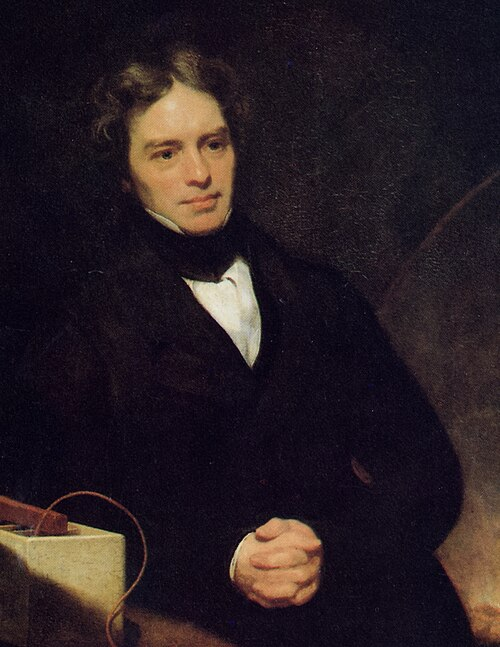
\includegraphics[width=\linewidth]{images/book3/faraday.jpg}
\end{minipage}\hfill
\begin{minipage}[t]{0.69\linewidth}
\vspace{0pt}
En 1834, Michael Faraday, mesurant les produits d'électrolyses avec un
voltamètre de sa conception, énonça que la masse d'une substance produite
à une électrode est proportionnelle à la quantité d'électricité qui a traversé le circuit, et
que, pour une quantité d'électricité donnée, les masses de substances différentes
sont dans le rapport de leurs équivalents chimiques. Il forgea les mots
électrode, anode, cathode, ion, anion et cation. La constante qui porte son
nom transforme ces lois en $Q = nF\,\Delta\xi$. (Portrait par Thomas Phillips,
1842, domaine public, Wikimedia Commons.)
\end{minipage}
\end{history}

\section{Piles de concentration}

\begin{definition}[Pile de concentration]\label{def:b2:cell-thermodynamics:concentration-cell}
Une \emph{pile de concentration}\index{pile de concentration} est formée de deux
demi-piles du même couple qui ne diffèrent que par la concentration (ou la
pression) d'une espèce.
\end{definition}

\begin{proposition}[Tension d'une pile de concentration]\label{prop:b2:cell-thermodynamics:concentration-cell}
Deux électrodes d'un métal M plongeant dans des solutions de \ce{M^{n+}} aux
concentrations $c_1 < c_2$, reliées par un pont salin, donnent une tension
\[
  U = \frac{RT}{nF}\ln\frac{c_2}{c_1} ,
\]
le pôle positif étant du côté le plus concentré. La pile fonctionne jusqu'à ce que les
deux concentrations soient égales.
\end{proposition}

\begin{proof}
D'après la relation de Nernst, chaque électrode a pour potentiel $E_i = E^\circ + (RT/nF)\ln c_i$ (\omterm{def:b2:chemical-potential:ideal-mixture}{solutions
diluées idéales})~; $E^\circ$ disparaît dans la différence. La réaction est
\ce{M^{n+}}(côté 2) $\to$ \ce{M^{n+}}(côté 1)~: du métal se dépose du
côté concentré (cathode) et se dissout du côté dilué (anode), ce qui
égalise les concentrations~; $\Delta_r G = RT\ln(c_1/c_2) < 0$ jusqu'à ce qu'elles soient
égales.
\end{proof}

\begin{omfigure}
\begin{tikzpicture}[font=\small, >={Stealth}]
  \pic at (0,0) {beaker={0.7}{omDef!10}};
  \pic at (3.6,0) {beaker={0.7}{omDef!32}};
  \pic at (-0.3,0.25) {electrode={black!25}};
  \pic at (3.9,0.25) {electrode={black!25}};
  \pic at (0.35,0.55) {saltbridge={2.9}};
  \pic (m) at (1.8,4.3) {meter={V}};
  % common (black) terminal on the anode side, red (+) on the cathode side
  \fill[black] (1.4,4.03) circle (0.065); \fill[red!70!black] (2.2,4.03) circle (0.065);
  \draw[thick] (-0.15,2.65) |- (m-a);
  \draw[thick] (4.05,2.65) |- (m-b);
  \node[anchor=east] at (-0.95,1.0) {\ce{Ag}};
  \node[anchor=west] at (4.45,1.0) {\ce{Ag}};
  \node at (0.25,-0.35) {\ce{Ag+} \qty{0.010}{mol/L}};
  \node at (3.6,-0.35) {\ce{Ag+} \qty{0.10}{mol/L}};
  \node[anchor=east] at (-0.9,2.3) {$-$ anode};
  \node[anchor=west] at (4.6,2.3) {cathode $+$};
  \node[font=\scriptsize] at (-0.1,-0.8) {\ce{Ag -> Ag+ + e-}};
  \node[font=\scriptsize] at (3.7,-0.8) {\ce{Ag+ + e- -> Ag}};
  \node[font=\scriptsize] at (1.8,5.05) {$U = \qty{59}{mV}$};
\end{tikzpicture}

{\small Une \omterm{def:b2:cell-thermodynamics:concentration-cell}{pile de concentration} à l'argent à \qty{25}{\degreeCelsius}. Le côté dilué est
l'anode~: l'argent s'y dissout et se dépose du côté concentré,
jusqu'à l'égalité des deux concentrations. $U = 0.0592\log(0.10/0.010) =
\qty{59}{mV}$.}
\end{omfigure}

Le même principe permet de mesurer des concentrations. Une électrode de verre, dont la fine
membrane sépare une solution de référence de l'échantillon, développe un potentiel de
membrane de $(RT/F)\ln 10 = \qty{59}{mV}$ par unité d'écart de pH à
\qty{25}{\degreeCelsius}~: le pH-mètre du volume de première année est une \omterm{def:b2:cell-thermodynamics:concentration-cell}{pile de concentration}
pour \ce{H+}. De part et d'autre de la membrane d'une cellule vivante, les concentrations inégales
de \ce{K+} créent de la même façon un potentiel de plusieurs dizaines de millivolts.

\section{Exercices}

\begin{exercise}[$\star$]\label{exo:b2:cell-thermodynamics:1}
À partir de $\Delta_f G^\circ(\ce{H2O}, \text{l}) = \qty{-237.14}{kJ/mol}$, calculer la
tension standard de la pile dihydrogène--dioxygène.
\end{exercise}

\begin{exercise}[$\star$]\label{exo:b2:cell-thermodynamics:2}
Une pile porte l'indication \qty{1.0}{A.h}. Calculer la charge qu'elle contient, en coulombs,
et la masse de zinc consommée à son anode (\ce{Zn -> Zn^2+ + 2e-}) lorsqu'elle est
entièrement déchargée.
\end{exercise}

\begin{exercise}[$\star$]\label{exo:b2:cell-thermodynamics:3}
Une pile Daniell délivre \qty{1.10}{V} à courant nul. Calculer $\Delta_r G$ pour une
mole de zinc et le travail électrique maximal pour \qty{10.0}{g} de zinc.
\end{exercise}

\begin{exercise}[$\star$]\label{exo:b2:cell-thermodynamics:4}
Deux électrodes de cuivre plongent dans des solutions de sulfate de cuivre(II) à \qty{1.0e-3}{mol/L}
et à \qty{0.10}{mol/L}. Calculer la tension à \qty{25}{\degreeCelsius} et indiquer les
pôles.
\end{exercise}

\begin{exercise}[$\star\star$]\label{exo:b2:cell-thermodynamics:5}
Une pile ($n = 2$) a pour $E^\circ = \qty{1.015}{V}$ et $dE^\circ/dT = \qty{-4.0e-4}{V/K}$
à \qty{298}{K} (données de l'exercice). Calculer $\Delta_r G^\circ$, $\Delta_r S^\circ$ et
$\Delta_r H^\circ$.
\end{exercise}

\begin{exercise}[$\star\star$]\label{exo:b2:cell-thermodynamics:6}
La pile de l'\cref{exo:b2:cell-thermodynamics:5} débite une mole de réaction
(a) de façon réversible~; (b) sous \qty{0.90}{V}. Calculer dans chaque cas le travail électrique et
la chaleur échangée avec le milieu extérieur.
\end{exercise}

\begin{exercise}[$\star\star$]\label{exo:b2:cell-thermodynamics:7}
Calculer $E^\circ(\ce{Fe^3+}/\ce{Fe})$ à partir des \omterm{def:b2:reaction-free-energy:gibbs-energy}{enthalpies libres} de formation
(\ce{Fe^2+} \qty{-78.90}{kJ/mol}, \ce{Fe^3+} \qty{-4.7}{kJ/mol}) et vérifier qu'il
est égal à $(E_1^\circ + 2E_2^\circ)/3$.
\end{exercise}

\begin{exercise}[$\star\star$]\label{exo:b2:cell-thermodynamics:8}
Calculer le potentiel standard du couple \ce{AgCl}/\ce{Ag}, puis le
potentiel d'une électrode au chlorure d'argent plongeant dans une solution de chlorure de potassium
à \qty{0.10}{mol/L}.
\end{exercise}

\begin{exercise}[$\star\star$]\label{exo:b2:cell-thermodynamics:9}
Les piles zinc--air utilisent \ce{2Zn + O2 -> 2ZnO} ($\Delta_f G^\circ(\ce{ZnO}) =
\qty{-318.30}{kJ/mol}$). Calculer la tension standard et l'énergie électrique
maximale, en \unit{kW.h}, par kilogramme de zinc.
\end{exercise}

\begin{exercise}[$\star\star\star$]\label{exo:b2:cell-thermodynamics:10}
Une pile à combustible à méthanol direct utilise \ce{CH3OH(l) + 3/2O2 -> CO2 + 2H2O(l)}. À partir de
$\Delta_f H^\circ$ (\unit{kJ/mol})~: \ce{CH3OH(l)} $-239$, \ce{CO2} $-393.51$,
\ce{H2O(l)} $-285.83$~; et de $S^\circ$ (\unit{J/(K.mol)})~: \ce{CH3OH(l)} 127.2,
\ce{CO2} 213.8, \ce{H2O(l)} 69.95, \ce{O2} 205.15, calculer $n$, $E^\circ$ et le
rendement maximal.
\end{exercise}

\begin{exercise}[$\star\star\star$]\label{exo:b2:cell-thermodynamics:11}
Une pile ($n = 2$) a pour $E = \qty{0.500}{V}$ et $dE/dT = \qty{+3.0e-4}{V/K}$ à
\qty{298}{K} (données de l'exercice). Montrer que, fonctionnant de façon réversible, elle fournit plus de
travail électrique que $-\Delta_r H$, et expliquer d'où vient l'énergie supplémentaire.
\end{exercise}

\begin{exercise}[$\star\star\star$]\label{exo:b2:cell-thermodynamics:12}
Deux électrodes à hydrogène (\qty{1}{bar} de \ce{H2}) plongent dans une solution de référence de
pH 7.00 et dans un échantillon. La tension vaut \qty{0.177}{V} à \qty{25}{\degreeCelsius},
la référence étant le pôle positif. Trouver le pH de l'échantillon, et expliquer
pourquoi le résultat ne dépend d'aucun potentiel standard.
\end{exercise}

\section{Problème~: le bus à pile à combustible}

\begin{problem}[{Problème du week-end --- la tension standard de la pile
dihydrogène--dioxygène à partir des enthalpies libres, son coefficient de température, le
rendement et la chaleur d'un empilement réel, et l'énergie d'un réservoir de dihydrogène}]
\label{pb:b2:cell-thermodynamics:1}
Un empilement de pile à combustible compte 400 cellules en série, chacune munie d'une membrane
échangeuse de protons (électrolyte acide). Données à \qty{298.15}{K} (CODATA, JANAF)~:
$\Delta_f H^\circ(\ce{H2O}, \text{l}) = \qty{-285.83}{kJ/mol}$, $\Delta_f
G^\circ(\ce{H2O}, \text{l}) = \qty{-237.14}{kJ/mol}$, $\Delta_f G^\circ(\ce{H2O},
\text{g}) = \qty{-228.58}{kJ/mol}$~; $S^\circ$ (\unit{J/(K.mol)})~: \ce{H2O(l)} 69.95,
\ce{H2} 130.68, \ce{O2} 205.15. $F = \qty{96485}{C/mol}$~; $M(\ce{H2}) =
\qty{2.016}{g/mol}$.
% ledger: dfh:H2O-l, janafG:H2O_l.298, janafG:H2O.298, s0:H2O_l, s0:H2_g, s0:O2_g, const:F, aw:H

\medskip
\noindent\textbf{Partie I --- La tension standard.}
\begin{enumerate}
  \item Écrire les demi-équations à l'anode et à la cathode, ainsi que la réaction
        de la pile.
  \item Combien d'électrons sont échangés par molécule de dihydrogène~?
  \item Calculer $E^\circ$ lorsque l'eau est formée à l'état liquide.
  \item Le calculer lorsque l'eau sort sous forme de vapeur.
  \item Expliquer la différence à l'aide de l'\omterm{def:b2:reaction-free-energy:gibbs-energy}{enthalpie libre} de vaporisation de l'eau.
  \item Calculer $\Delta_r H^\circ$ et le rendement maximal à \qty{298}{K}.
\end{enumerate}

\medskip
\noindent\textbf{Partie II --- La température.}
\begin{enumerate}[resume]
  \item Calculer $\Delta_r S^\circ$ pour l'eau liquide.
  \item En déduire $dE^\circ/dT$.
  \item Estimer $E^\circ$ à \qty{80}{\degreeCelsius}, la température de fonctionnement de
        l'empilement.
  \item Comparer le résultat de cette méthode à la valeur JANAF à \qty{400}{K}, $\Delta_f
        G^\circ(\ce{H2O}, \text{l}) = \qty{-221.01}{kJ/mol}$.
  \item Quelle chaleur la pile réversible échange-t-elle par mole de dihydrogène à
        \qty{298}{K}~? Est-elle reçue ou cédée~?
  \item Estimer le rendement maximal à \qty{80}{\degreeCelsius}.
\end{enumerate}

\medskip
\noindent\textbf{Partie III --- L'empilement réel sous \qty{0.70}{V} par cellule.}
\begin{enumerate}[resume]
  \item Calculer le travail électrique par mole de dihydrogène.
  \item Calculer le rendement rapporté à $\Delta_r H^\circ$ et à $\Delta_r G^\circ$.
  \item Calculer la chaleur libérée par mole de dihydrogène.
  \item Quelle part en est inévitable, et quelle part est due au courant~?
  \item L'empilement débite \qty{300}{A}. Calculer la consommation de dihydrogène d'une
        cellule, puis de l'empilement, en moles et en grammes par seconde.
  \item Calculer la puissance électrique de l'empilement.
  \item Calculer la puissance thermique que doit évacuer le circuit de refroidissement.
\end{enumerate}

\medskip
\noindent\textbf{Partie IV --- Le réservoir.}
\begin{enumerate}[resume]
  \item Quelle quantité de dihydrogène contiennent \qty{5.0}{kg}~?
  \item Quelle charge traverse les cellules, comptée sur l'ensemble d'entre elles, lorsque
        ce dihydrogène est oxydé~?
  \item Calculer l'énergie électrique fournie par l'empilement, chaque cellule étant sous
        \qty{0.70}{V}.
  \item La convertir en kilowattheures.
  \item Pendant combien de temps l'empilement peut-il fournir la puissance de la question 18~?
  \item Donner l'énergie électrique fournie par \qty{5.0}{kg} de dihydrogène sous
        \qty{0.70}{V} par cellule.
\end{enumerate}
\end{problem}
